\documentclass[onecolumn]{article}
\usepackage{graphicx} % Required for inserting images
\usepackage{amsmath}
\usepackage{amsfonts}
\usepackage{pythonhighlight}
\usepackage{datetime}
\usepackage{subcaption}
\usepackage{titling}
\usepackage{matlab-prettifier}
\usepackage[a4paper, total={6in, 8in}]{geometry}

\footskip = 1pt
\textheight = 700pt
\setlength{\droptitle}{-10em}

\title{IN3170 - Lab 2}
\author{Andreas Engøy, Erik Røset \& Daniel Tran}
\date{\monthname[\the\month] \the\year}

\begin{document}
\maketitle

\section*{Introduction}
This lab rapport details the two tasks for Lab 2 in the course IN3170 Microelectronics. In the first task a double inverter circuit is built in order to probe, measure and calculate different characteristics of the circuit. In the second task [ONE SENTENCE DESCRIPTION OF TASK 2]

\section*{Experimental}
\subsection*{Equipment}
\begin{table}[h!]
    \centering
    \begin{tabular}{|c|c|c|}
        \hline
        \textbf{Component} & \textbf{Model} & \textbf{Quantity} \\
        \hline
        Resistor & 100k$\Omega$ & 1 \\
        Hex Inverter IC & 74HCT14 & 1 \\
        Copper wires & - & 12 \\
        Printed Circuit Board & - & 1 \\
        Soldering iron & - & 1 \\
        Soldering wire & - & 1 \\
        Oscilloscope & HP54622 & 1 \\
        Waveform generator  & HP33120 & 1 \\
        Voltage source & HPE3631 & 1 \\ 
        \hline
    \end{tabular}
    \caption{List of components used in the experiment.}
    \label{tab:bom}
\end{table}

\begin{figure}[h!]
    \centering
    \begin{subfigure}{.5\textwidth}
      \centering
      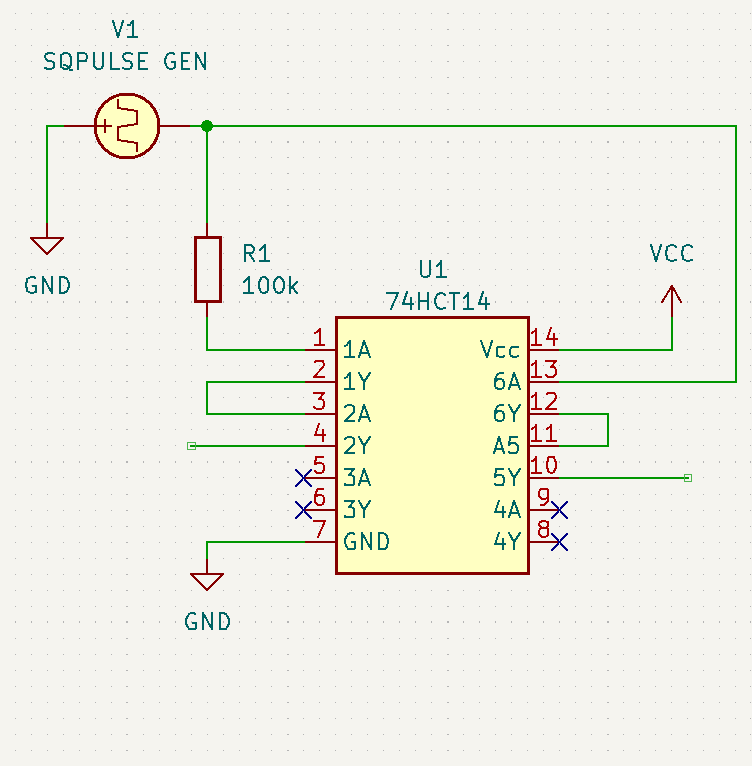
\includegraphics[width=.78\linewidth]{Task 1 Circuit.png}
      \caption{Circuit diagram}
      \label{fig:sub1}
    \end{subfigure}%
    \begin{subfigure}{.5\textwidth}
      \centering
      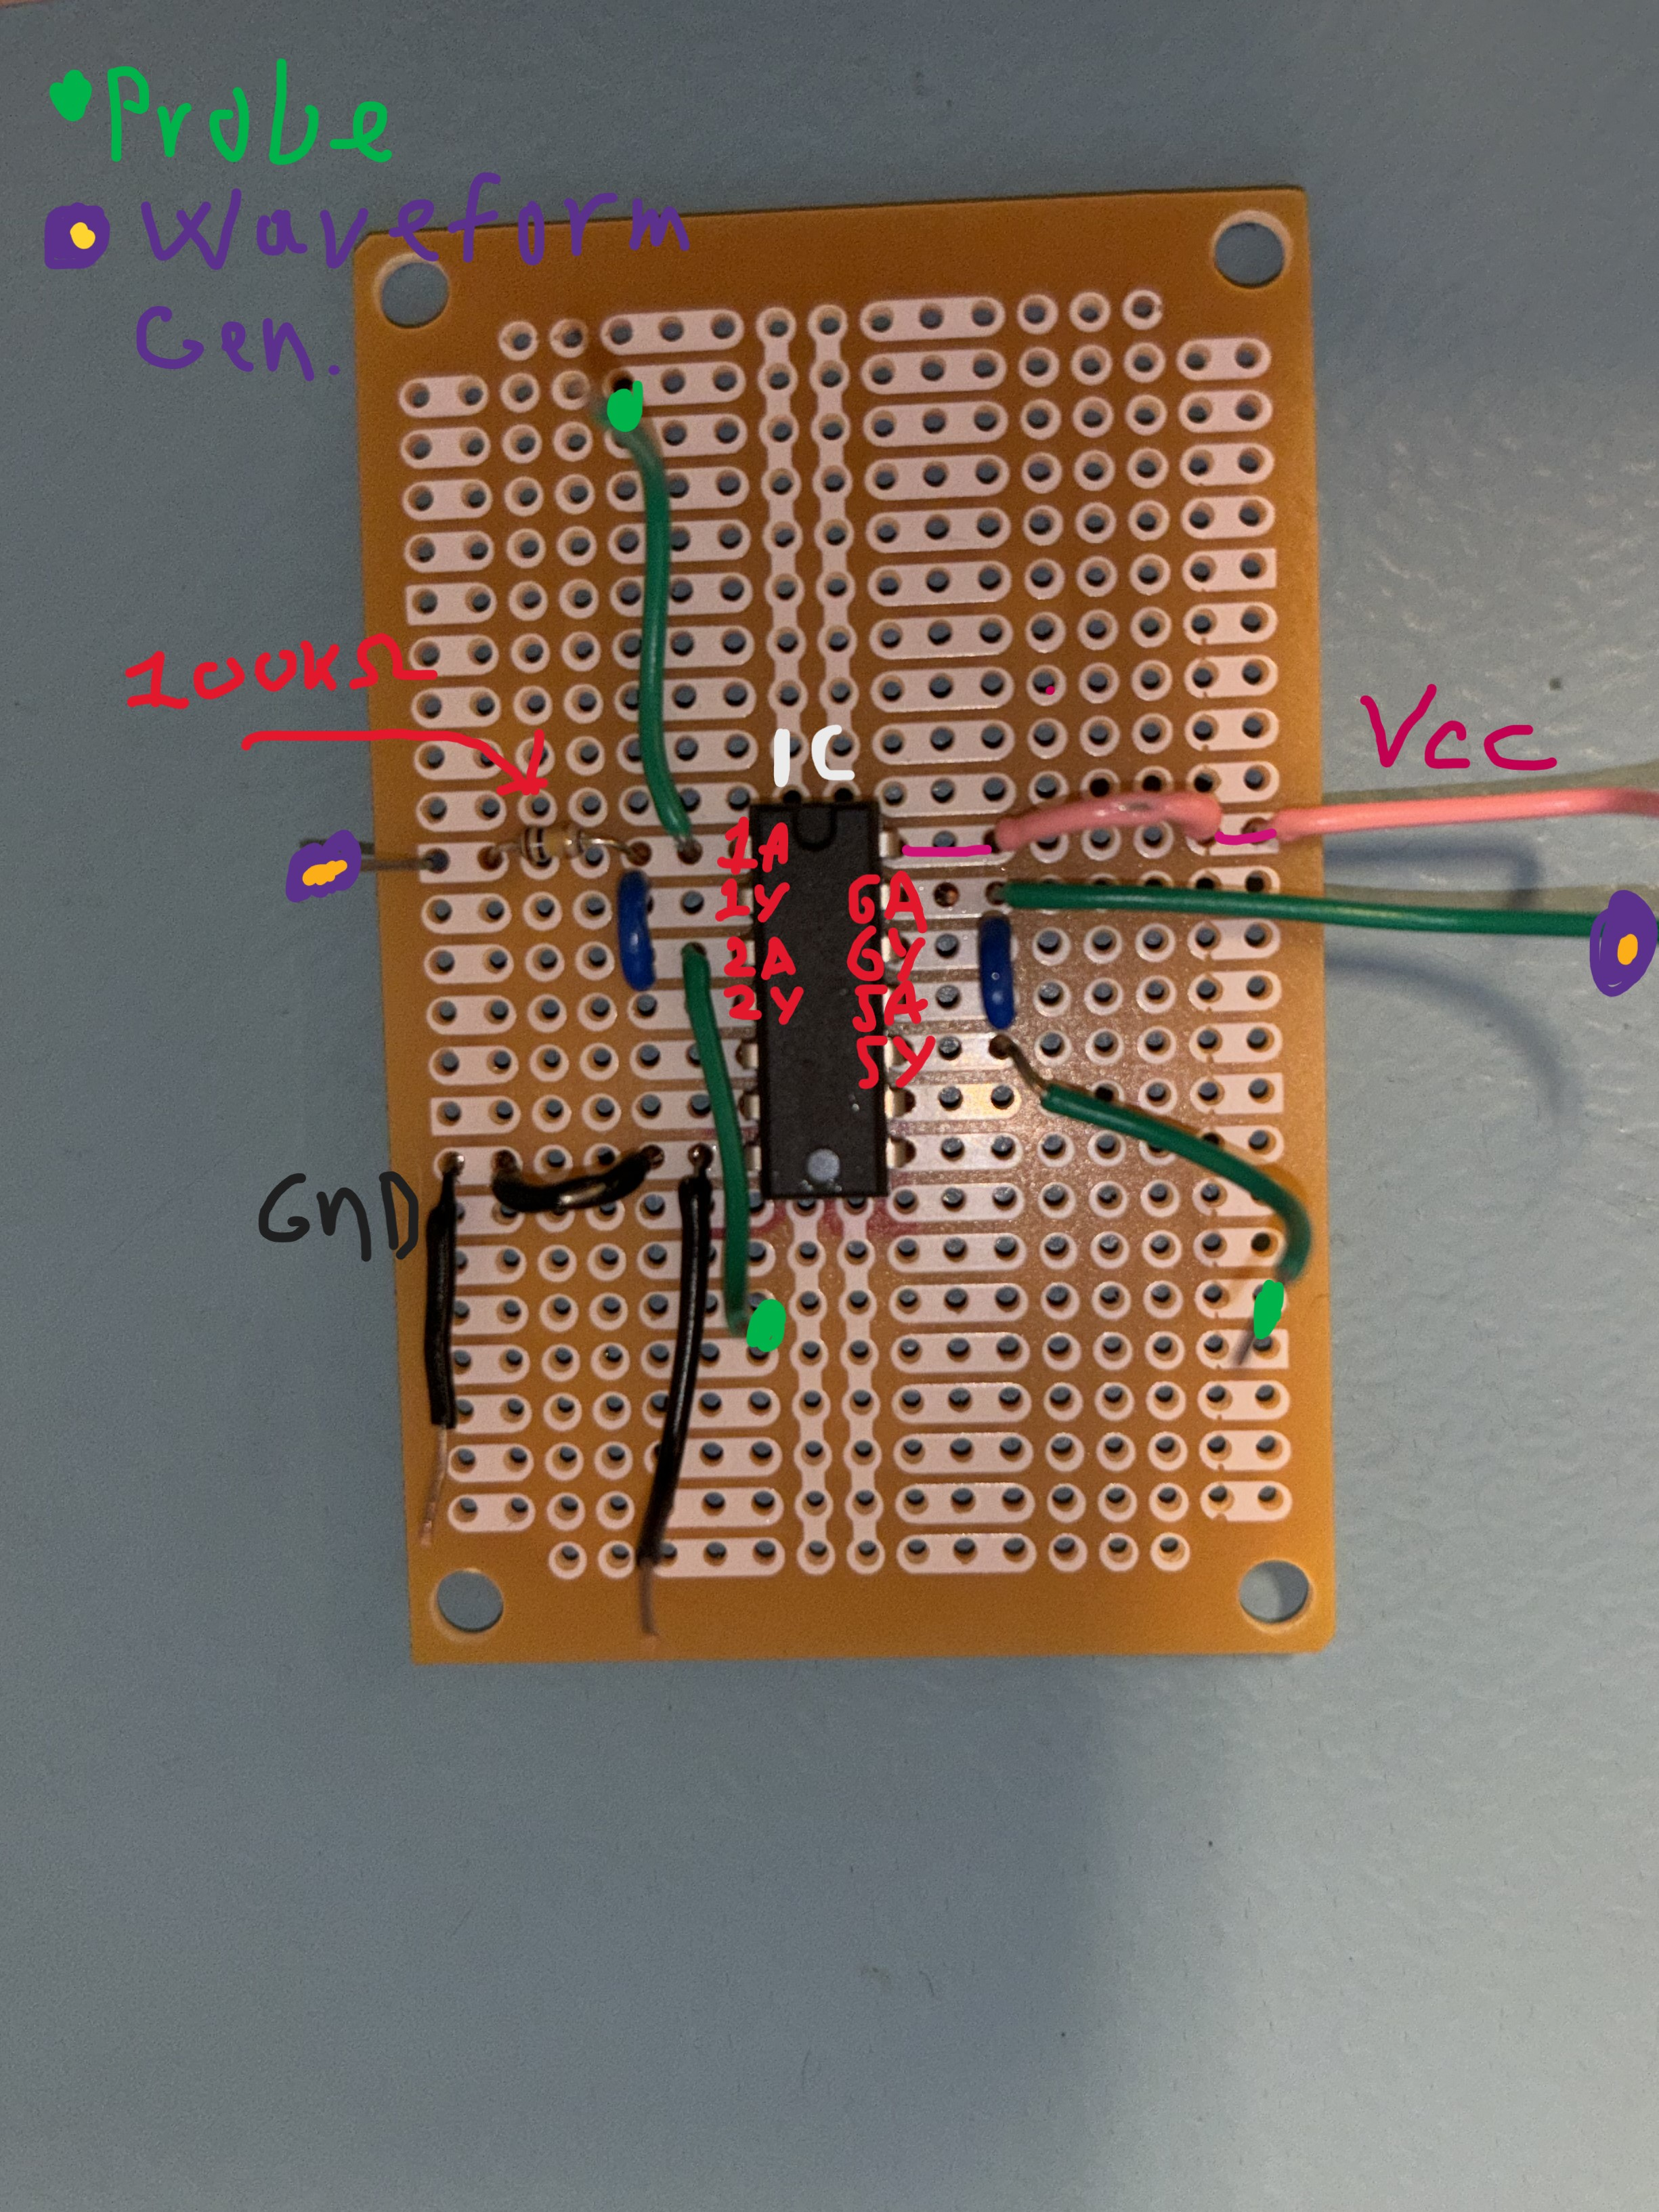
\includegraphics[width=.6\linewidth]{Photo of circuit.jpg}
      \caption{Photo of the circuit}
      \label{fig:sub2}
    \end{subfigure}
    \caption{Schematic and photo of two double inverters connected in series.}
    \label{fig:test}
    \end{figure}
\section*{Results}
\section*{Appendix}

\end{document}